% \documentclass is book
\documentclass[12pt,twoside,letterpaper,openany]{book}

\usepackage[utf8]{inputenc}
\usepackage{ifthen}                     % provide if-then-else operators
\usepackage{datetime}
\usepackage{textcomp}
\usepackage{pdflscape}

% --------------------------------------------------------------------------
% Global variables required in document formatting
% --------------------------------------------------------------------------
%
% BOOK MODE
%
\newboolean{bookmode}                  % boolean used to control book format
% Ensure that only one of the next two lines is active:
\setboolean{bookmode}{true}           % turn book mode on
%\setboolean{bookmode}{false}           % turn book mode off

%
% DRAFT MODE
%
\newboolean{draftmode}                  % boolean used to control draft-mode
% Ensure that only one of the next two lines is active:
%\setboolean{draftmode}{true}            % turn draft mode on
\setboolean{draftmode}{false}           % turn draft mode off
% --------------------------------------------------------------------------
%
% GENERAL AUTHOR, TITLE AND KEYWORDS
%
% Nombre del Estudiante
\newcommand{\scriptAuthor}{Luis Pedro Morales Rodríguez}

% Título de la tesis
\newcommand{\scriptTitleSpanish}{Implementación de un sistema embebido para control de acceso en gimnasios mediante reconocimiento facial}
\newcommand{\scriptTitle}{Implementation of an embedded system for access control in gyms using facial recognition}

% Keywords
\newcommand{\scriptKeywords}{PALABRAS CLAVE}

% Descripción de la editorial
\newcommand{\boxeditorial}{%
}

\newcommand{\spanishplacedate}{Cartago, \ifcase\month \or enero\or febrero\or marzo\or abril\or mayo\or junio\or julio\or agosto\or septiembre\or octubre\or noviembre\or diciembre\fi \space 
de \number\year}
\newcommand{\placedate}{Cartago, \monthname, \number \year}

% Para el PDF (cambiar si se desea otras cosas a lo indicado arriba
\newcommand{\pdfAuthor}{\scriptAuthor}
\newcommand{\pdfTitle}{\scriptTitle} 
\newcommand{\pdfKeywords}{\scriptKeywords}

% --------------------------------------------------------------------------

% include all packages and define all required general macros
%%%%%%%%%%%%%%%%%%%%%%%%%%%%%%%%%%%%%%%%%%%%%%%%%%%%%%%%%%%%%%%%%%%%%%%%%%%%%%%
% Author:  Pablo Alvarado
%
% Escuela de Electrónica
% Instituto Tecnológico de Costa Rica
%
% Phone:   +506 550 2106
% Fax:     +506 591 6629
% email:   palvarado@ietec.org
%
% $Id: macros.tex 1497 2010-08-09 17:04:26Z palvarado $
%
%%%%%%%%%%%%%%%%%%%%%%%%%%%%%%%%%%%%%%%%%%%%%%%%%%%%%%%%%%%%%%%%%%%%%%%%%%%%%%%

% Configuration of the exercises package, which is used to collect all
% problems and answers in the document.
\usepackage[exercisedelayed,answerdelayed,lastexercise]{exercise}
\renewcounter{Exercise}[chapter]
\renewcommand{\ExerciseName}{Problema}
\renewcommand{\theExercise}{\thechapter.\arabic{Exercise}}
\newcommand{\ExerciseLabel}{Exercise.\theExercise}
\renewcommand{\ExerciseHeader}%
{\textbf{\ExerciseName\ \theExercise.\ \ExerciseHeaderTitle\ }}
\renewcommand{\AnswerHeader}%
{\textbf{\ExerciseName\ \theExercise.\ }}


\usepackage{ifpdf}

% Command to change between draft or release mode:
\newcommand{\ifdraft}[2]{\ifthenelse{\boolean{draftmode}}{#1}{#2}}
% Command to change between draft or release mode:
\newcommand{\ifbook}[2]{\ifthenelse{\boolean{bookmode}}{#1}{#2}}

% include all required packages here
\usepackage[spanish,english]{babel}     % supports english, but default is 
                                        % spanish...
\newcommand*{\SelectSpanish}{%          % well, the last line indeed selects
  \hyphenrules{spanish}%                % english over spanish, but with this
  \languageshorthands{spanish}%         % command we turn it around.
  \captionsspanish                      % The reason: hyperref has some
  \datespanish                          % problems with the spanish babel,
}                                       % so we use some trick here so that it
\AtBeginDocument{\SelectSpanish}        % thinks it is english.

\usepackage{makeidx}                    % to create index file

\ifdraft{%
  %\usepackage[refpage]{nomencl}        % Use to easily administrate the list
 \usepackage{nomencl}                   % of symbols
}{%
 \usepackage{nomencl}
}
%\usepackage{times}                     % replace latex pk fonts with ps type I
                                        % don't forget to use dvips -D600 -Pcmz
                                        % to ensure Type I fonts!
\usepackage{amsmath}
\usepackage{amssymb,amstext}            % AMS-math and symbols package
\usepackage{mathrsfs}                   % Calygraphic fonts for transforms
\usepackage{array}                      % extensions to tabular environment
\usepackage{longtable}                  % supports extraordinary long tables
\usepackage{tabularx}                   % supports tables with fixed width
\usepackage{afterpage}                  % put something only after the page
\usepackage{multirow}                   % supports multiple row grouping in 
                                        % tables
\usepackage{multicol}                   % multiple columns environments
\usepackage{paralist}                   % a few enumeration settings

\usepackage[hang,%
            small,%
            bf]{caption}                % nicer figure captions
%\usepackage{sty/ftcap}                 % switch \abovecaptionskip and
%                                       % \belowcaptionskip for tables, in 
%                                       % order to avoid the caption to be
%                                       % too near to the table itself
% locally added packages
\usepackage{float}                      % really place figures "here" (H)
\usepackage{booktabs}                   % book type tabulars

% the own style with options depending on the draft mode
\ifdraft{%
\usepackage[todo]{sty/tecStyle}         % some command definitions
                                        % options [todo] todo-index
}{%
\usepackage{sty/tecStyle}               % some command definitions
                                        % options [todo] todo-index
}

%% fix the title for examples
\renewcommand{\examplelistname}{Índice de ejemplos}
\renewcommand{\examplename}{Ejemplo}


\usepackage{url}                        % allows linebreaks at certain
                                        % characters or combinations of 
                                        % characters for URLs

\usepackage[nottoc]{tocbibind}          % Fix the hyperrefs to TOC,TOF, etc.
                                        % and ensure that they appear all in 
                                        % the Table of Contents

\usepackage{color}                      % Support for colors
\definecolor{dkred}{rgb}{0.5,0,0}       %   dark red
\definecolor{dkgreen}{rgb}{0,0.3,0}     %   dark green
\definecolor{dkblue}{rgb}{0,0.0,0.5}    %   dark blue
\definecolor{dkgray}{gray}{0.4}         %   dark gray
\definecolor{dkmagenta}{rgb}{0.3,0.0,0.3} % dark magenta
\definecolor{ltyellow}{rgb}{1.0,1.0,0.7}  % light yellow

\newcommand{\bG}[1]{\textcolor{dkgreen}{\textbf{#1}}}
\newcommand{\bR}[1]{\textcolor{dkred}{\textbf{#1}}}
\newcommand{\bB}[1]{\textcolor{dkblue}{\textbf{#1}}}
\newcommand{\bM}[1]{\textcolor{dkmagenta}{\textbf{#1}}}
\newcommand{\bY}[1]{\textcolor{dkyellow}{\textbf{#1}}}
\newcommand{\bC}[1]{\textcolor{dkcyan}{\textbf{#1}}}

% For pdflatex
% - The hyperref package should always be loaded last, since it has to
%   overwrite some of the commands.
% - The package subfigure caused that the pagebackrefs and index refs were set
%   incorrectly.

\ifpdf
%
% final / draft document options
\usepackage[pdftex,final]{graphicx}     % for inserting pdf-graphics.
                                        % options final / draft
\ifdraft{%

\usepackage[pdftex,%
            pdftitle={\pdfTitle},%
            pdfauthor={\pdfAuthor},%
            pdfsubject={Notas de Clase},%
            pdfkeywords={\pdfKeywords},%
            naturalnames=true,
            linktocpage,
            hyperindex,
            colorlinks,
            urlcolor=dkred,          %\href to external url
            filecolor=dkmagenta,     %\href to local file
            linkcolor=dkred,         %\ref and \pageref
            citecolor=dkgreen,       %\cite
            pagecolor=dkred,
            pagebackref,
            plainpages=false,
            pdfpagelabels,
            pdfpagemode=UseOutlines, % means use bookmarks (None,UseOutlines)
            % bookmarksopen=false,   % would show the whole hierarchy if true
            bookmarksnumbered=true,
            pdfpagelayout=OneColumn, % SinglePage,OneColumn,TwoColumnLeft,...
            pdfview=FitH, % FitB,FitBH,FitBV,Fit,FitH,FitV
            pdfstartview=FitH, % FitB,FitBH,FitBV,Fit,FitH,FitV
            ]{hyperref}
}{%
\usepackage[pdftex,%
            pdftitle={\pdfTitle},%
            pdfauthor={\pdfAuthor},%
            pdfsubject={Notas de clase},%
            pdfkeywords={\pdfKeywords},%
            naturalnames=true,
            linktocpage,hyperindex,
            colorlinks,
            urlcolor=dkred,          %\href to external url
            filecolor=dkmagenta,     %\href to local file
            linkcolor=dkred,         %\ref and \pageref
            citecolor=dkgreen,       %\cite
            pagecolor=dkred,
            % pagebackref,           % only in draft modus should this be on.
            plainpages=false,
            pdfpagelabels,
            pdfpagemode=UseOutlines, % means use bookmarks (None,UseOutlines)
            % bookmarksopen=false,   % open the whole hierarchy if true!
            bookmarksnumbered=true,
            pdfpagelayout=OneColumn, % SinglePage,OneColumn,TwoColumnLeft,...
            pdfview=FitH, % FitB,FitBH,FitBV,Fit,FitH,FitV
            pdfstartview=FitH, % FitB,FitBH,FitBV,Fit,FitH,FitV
            ]{hyperref}
}

%
% Ensure that the links of the images point to the top of the images and not
% to the caption
%
\usepackage[figure]{hypcap}

% %
% % Ensure that pdfLaTeX do the same spacing as LaTeX
% %
\pdfadjustspacing=1 
% %
\else   % i.e. if not pdf

\usepackage[active]{srcltx}             % insert links into the dvi to jump
\usepackage[dvips,final]{graphicx}      % for inserting eps-graphics.
                                        % options final / draft
                                        % into the sources directly.
\ifdraft{%
\usepackage[ps2pdf,%
            pdftitle={\pdfTitle}%
            pdfauthor={\pdfAuthor},%
            pdfsubject={Notas de clase},%
            pdfkeywords={\pdfKeywords},%
            % plainpages=false,
            linktocpage,
            hyperindex,
            pagebackref,
            % pdfpagelabels,
            pdfpagemode=UseOutlines,
            pdfstartview=FitH]{hyperref}
}{%
\usepackage[ps2pdf,%
            pdftitle={\pdfTitle}%
            pdfauthor={\pdfAuthor},%
            pdfsubject={Notas de clase},%
            pdfkeywords={\pdfKeywords},%
            % plainpages=false,
            linktocpage,
            hyperindex,
            % pagebackref,
            % pdfpagelabels,
            pdfpagemode=UseOutlines,
            pdfstartview=FitH]{hyperref}
}

%\usepackage[ps2pdf]{hyperref}

\fi  % end of if pdf or not

\usepackage{sty/algorithmic}            % algorithmic environment


\usepackage{rotating}                   % allow block rotation


%%%%%%%%%%%%%%%%%%%%%%%%%%%%%%%%%%%%%%%%%%%%%%%%%%%%%%%%%%%%%%%%%%%%%%%%%%%%%%%

%\sloppy

%
% Some own font definitions
%
\DeclareMathAlphabet{\mathpzc}{OT1}{pzc}{m}{it}
\DeclareMathAlphabet{\mathpss}{OT1}{cmss}{m}{sl}

%
% page layout
%

\usepackage{vmargin}
\setpapersize{USletter}

% For letter-paper printing
\setmarginsrb{33mm}{8mm}{23mm}{7mm}{15pt}{15pt}{7mm}{12mm}
%\setlength{\headheight}{15pt}         % fancy headers wanted this

%
% Fraction of Float Object / Text
%

\renewcommand{\topfraction}{0.95}       % how much of top of page should be 
                                        % allowed to be float object?
\renewcommand{\bottomfraction}{0.95}    % how much of bottom of page should be
                                        % allowed to be float object?
\renewcommand{\textfraction}{0.05}      % how much of page must be text?

\usepackage{fancyhdr}                   % fancy page headers

\usepackage{lastpage}

%
% header and footer layout (needs package fancyhdr)
%
\newcommand{\copyrightfooter}{\tiny{\copyright 2005-2010 --- P.~Alvarado %
    \qquad Uso exclusivo ITCR}}
%
\newcommand{\draftfoot}%
  {\ifdraft{\textcolor{dkblue}{\tiny\textsl{Borrador: \today}}{}}
           {}
}

\pagestyle{fancy}
\renewcommand{\chaptermark}[1]{\markboth{{\small
    \thechapter\hspace*{1mm}#1}}{}}
\renewcommand{\sectionmark}[1]{\markright{{\small
    \thesection\hspace*{1mm}#1}}{}}
\lhead[{\small\textbf\thepage}]{\fancyplain{}%
        {{\slshape \small\nouppercase{\leftmark}}}}
\chead[]{}
\rhead[\fancyplain{}%
        {{\slshape \small\nouppercase{\rightmark}}}]{{\small\textbf\thepage}}
\lfoot[]{\draftfoot}
\ifbook{%
  \cfoot[]{}
}{
  \cfoot[\copyrightfooter]{\copyrightfooter}
}
\rfoot[\draftfoot]{}
\renewcommand{\headrulewidth}{0.5pt}
\renewcommand{\footrulewidth}{0pt}

%
% Caption style for tables
% Requires the packages caption2 and ftcap
% (caption2 required this, but is obsolete now:)
%
%\newcaptionstyle{tablecaptionstyle}{%
%  \renewcommand\captionlabelfont{\normalsize\bf}
%  \renewcommand\captionfont{\normalsize}
%  \usecaptionstyle{hang}%
%}

% For caption v3:
\captionsetup[table]{position=top,format=hang,textfont={normalsize},labelfont={normalsize,bf}}

\newcommand{\tablecaption}[2][foo]{%
  \ifthenelse{\equal{#1}{foo}}{%
    %\captionstyle{tablecaptionstyle}%
    \caption{#2}%
  }
  {%
    %\captionstyle{tablecaptionstyle}%
    \caption[#1]{#2}%
  }
}
\addto\extrasspanish{\renewcommand{\tablename}{Tabla}}
\addto\extrasspanish{\renewcommand{\listtablename}{\'Indice de tablas}}

%
% paragraph layout
%
\renewcommand{\baselinestretch}{1.1}    % line spacing
\parindent0em                           % indentation width of first line
\parskip1.3ex                           % space between paragraphs

%
% document consists of
% chapter - section - subsection - subsubsection - paragraph - subparagraph
%
\setcounter{secnumdepth}{2}             % depth of section numbering
\setcounter{tocdepth}{2}                % depth of table of contents

%
% prepares index from entries like \index{word} or \index{group!word}.
% don't forget to call "makeindex filename" for final index generation.
%
\makeindex                            %% for package makeidx.sty
%\newindex{default}{idx}{ind}{Index}  %% for package index.sty

\newcommand{\octave}{GNU/Octave}


%
% prepares notation or nomenclature 
%
%\makeglossary
\makenomenclature

%%% Local Variables: 
%%% mode: latex
%%% TeX-master: "main"
%%% End: 



\usepackage{listings}
\definecolor{mauve}{rgb}{0.58,0,0.82}
\lstset{frame=tb,
  language=Java,
  aboveskip=3mm,
  belowskip=3mm,
  showstringspaces=false,
  columns=fullflexible,
  basicstyle={\small\ttfamily},
  numbers=none,
  numberstyle=\tiny\color{gray},
  keywordstyle=\color{blue},
  commentstyle=\color{dkgreen},
  stringstyle=\color{mauve},
  breaklines=true,
  breakatwhitespace=true,
  tabsize=3,
  literate=
    {á}{{\'a}}1
    {é}{{\'e}}1
    {í}{{\'i}}1
    {ó}{{\'o}}1
    {ú}{{\'u}}1
}

\lstdefinestyle{TextoEjemplo}{keywordstyle=\color{black}, stringstyle=\color{black}}

\lstdefinestyle{TextoEjemploJSON}{breaklines=true}
\usepackage{subfig}
\usepackage{caption}

%Para generar una numeración continua de las imagenes y tablas
\usepackage{chngcntr}
\counterwithout{figure}{chapter}
\counterwithout{table}{chapter}

\usepackage{cleveref}

\usepackage{pdfpages}

% Load graphicx with draft/final option based on draftmode
\ifthenelse{\boolean{draftmode}}
  {\usepackage[draft]{graphicx}}
  {\usepackage{graphicx}}

\usepackage{tikz}
\usetikzlibrary{mindmap}

% allow equations to be splitted (breaked) into several pages
\allowdisplaybreaks[3]

% --------------------------------------------------------------------------
\begin{document}
  % where to look for graphics
  \graphicspath{{./}{./fig/}}

  \pagenumbering{alph}
  % fix some terms not activated due to the bug of hyperref with spanish.
  \renewcommand{\tablename}{Tabla}
  \renewcommand{\listtablename}{\'Indice de tablas}
  \renewcommand{\examplesolution}{Solución}
  \pagestyle{empty}

  
\thispagestyle{empty} 

\begin{center}

{\large\bf{Tecnológico de Costa Rica}}

\par\vspace{1ex}

{\large\bf{Escuela de Ingeniería en Computadores}}\\
{\normalsize (Computer Engineering School)}

\par\vspace{20mm}

{\large\bf{Programa de Licenciatura en Ingeniería en Computadores}} \\
{\normalsize (Licentiate Degree Program in Computer Engineering)}

\par\vspace{20mm}


\includegraphics[width=9.5cm]{fig/logo-tec.png}

\par\vspace*{\fill}

{\large\bf{\scriptTitleSpanish}}
\\
{\normalsize (\scriptTitle)}


\par\vspace*{\fill}

{\large Informe de Trabajo de Graduación para optar por el título de Ingeniero en Computadores con grado académico de Licenciatura}\\
{\scriptsize(Report of Graduation Work in fulfillment of the requirements for the degree of Licentiate in Computer Engineering)}


\par\vspace{20mm}

\scriptAuthor

\vspace*{\fill}


\normalsize {\spanishplacedate} \\
\scriptsize {(\placedate)}


\end{center}
\newpage 



%%% Local Variables: 
%%% mode: latex
%%% TeX-master: "main"
%%% End: 
                                 % Titlepage
  
  %Página con la nota \includepdf[pages=-, offset=75 -75]{Acta.pdf}
  
  %\cleardoublepage
  \thispagestyle{empty}

\rule{10mm}{0pt}

\vfill

Declaro que el presente Proyecto de Graduación ha sido realizado enteramente
por mi persona, utilizando y aplicando literatura referente al tema e
introduciendo conocimientos propios.

En los casos en que he utilizado bibliografía he procedido a indicar las
fuentes mediante las respectivas citas bibliográficas.  En consecuencia,
asumo la responsabilidad total por el trabajo de graduación realizado y por
el contenido del correspondiente informe final.



\vspace*{8mm}

\begin{flushright}
  \scriptAuthor\par
  Cartago, \today \par
  Céd: 9-0109-0674
\end{flushright}



%%% Local Variables: 
%%% mode: latex
%%% TeX-master: "main"
%%% End: 

  %\cleardoublepage
  \thispagestyle{empty}

%%
%% Indique los nombres de los lectores y asesor
\newcommand{\lectorI}{}
\newcommand{\lectorII}{}
\newcommand{\director}{Pedro Gutiérrez García}


\begin{center}
  \begin{tabular}{c}
    Instituto Tecnológico de Costa Rica \\
    Área Académica de Ingeniería en Computadores \\
    Proyecto de Graduación \\
    Tribunal Evaluador
  \end{tabular}
\end{center}

\vfill

Proyecto de Graduación defendido ante el presente Tribunal Evaluador como 
requisito para optar por el título de Ingeniero en Computadores con el grado 
académico de Licenciatura, del Instituto Tecnológico de Costa Rica.  

\vfill

\vspace*{20mm}
\begin{center}
 Miembros del Tribunal
\end{center}
\vspace*{8mm}

\vfill

\begin{center}
  \begin{tabular}{ccc}
    \rule{70mm}{0.5pt} & \rule{15mm}{0pt} & \rule{70mm}{0.5pt} \\
    \lectorI && \lectorII \\
    Profesor Lector && Profesor Lector
  \end{tabular}
  
  \vspace{10mm}

  \begin{tabular}{c}
    \rule{6cm}{0.5pt} \\
    \director \\
    Profesor Asesor
  \end{tabular}
\end{center}

\vfill


Los miembros de este Tribunal dan fe de que el presente trabajo de graduación
ha sido aprobado y cumple con las normas establecidas por el Área Académica de Ingeniería en Computadores.

\vfill

\begin{center}
  \spanishplacedate\par
\end{center}

%\cleardoublepage

%%% Local Variables: 
%%% mode: latex
%%% TeX-master: "main"
%%% End: 

  \thispagestyle{empty}

%%
%% Los nombres de lectores y asesor se definen en el archivo tribunal.tex
%%

\begin{center}
  \begin{tabular}{c}
    Instituto Tecnológico de Costa Rica \\
    Área Académica de Ingeniería en Computadores \\
    Proyecto de Graduación \\
    Tribunal Evaluador \\
    Acta de Evaluación
  \end{tabular}
\end{center}

\vfill

Proyecto de Graduación defendido ante el presente Tribunal Evaluador como 
requisito para optar por el título de Ingeniero en Computadores con el grado 
académico de Licenciatura, del Instituto Tecnológico de Costa Rica.  

\vspace*{15mm}

\begin{center}
  Estudiante: \emph{\scriptAuthor} 
\end{center}

\vfill

\begin{center}
  Nombre del Proyecto: \emph{\scriptTitleSpanish}
\end{center}

\vspace*{20mm}
\begin{center}
 Miembros del Tribunal
\end{center}
\vspace*{8mm}

\vfill

\begin{center}
  \begin{tabular}{ccc}
    \rule{70mm}{0.5pt} & \rule{15mm}{0pt} & \rule{70mm}{0.5pt} \\
    \lectorI && \lectorII \\ %% Nombres definidos en tribunal.tex
    Profesor Lector && Profesor Lector
  \end{tabular}
  
  \vspace{10mm}

  \begin{tabular}{c}
    \rule{6cm}{0.5pt} \\
    \director \\ %% Definido en tribunal.tex
    Profesor Asesor
  \end{tabular}
\end{center}

\vfill

Los miembros de este Tribunal dan fe de que el presente trabajo de graduación
ha sido aprobado y cumple con las normas establecidas por el Área Académica de Ingeniería en Computadores.

\vfill

\begin{center}
  Nota final del Proyecto de Graduación: \rule{3cm}{0.5pt}
\end{center}
\vfill

\begin{center}
  \spanishplacedate\par
\end{center}

\cleardoublepage

%%% Local Variables: 
%%% mode: latex
%%% TeX-master: "main"
%%% End: 

  \chapter*{Resumen}
\thispagestyle{empty}



\bigskip

\textbf{Palabras clave:} \scriptKeywords

\clearpage
\chapter*{Abstract}
\thispagestyle{empty}



\bigskip

\textbf{Keywords:}

\cleardoublepage

%%% Local Variables: 
%%% mode: latex
%%% TeX-master: "main"
%%% End: 

  \vspace*{0.4\textheight}
{\hfill{\Large{\emph{DEDICATORIA}}}}

  \chapter*{Agradecimientos}
\thispagestyle{empty}


\vspace*{1cm}

\scriptAuthor

Cartago, \today

\cleardoublepage

%%% Local Variables: 
%%% mode: latex
%%% TeX-master: "paMain"
%%% End: 


  %----------------------------------------------------------------------------
  \frontmatter
  %----------------------------------------------------------------------------
  \pagestyle{fancy}

  \pdfbookmark[1]{Indice General}{Indice General}

  \parskip0ex                           % space between paragraphs

\renewcommand{\figurename}{Fig.}
\renewcommand{\figureautorefname}{Fig.}
\renewcommand{\autoref}[1]{\hyperref[#1]{\figureautorefname~\ref*{#1}}}
  \tableofcontents                                      % Table of contents
  %\listoffigures                                        % List of figures
  {
    \let\oldnumberline\numberline
    \renewcommand{\numberline}{Fig.~\oldnumberline}
    \listoffigures
  } 
  %\listoftables                                         % List of tables
    {
    \let\oldnumberline\numberline
    \renewcommand{\numberline}{Tabla~\oldnumberline}
    \listoftables
  } 
\ifdraft{%
  % todo's                                              % TODOs
  \listoftodo
}{%
}

  %% ---------------------------------------------------------------------------
%% paNotation.tex
%%
%% Notation
%%
%% $Id: notation.tex 1467 2010-07-24 16:47:17Z palvarado $
%% ---------------------------------------------------------------------------

\newcommand{\nms}{\negmedspace}

%%
% Commands required for the nomenclature groups
%
% There are following prefix forms:
%  a   abbreviation    \syma[key]{symbol}{description}
%  g   general         \symg[key]{symbol}{description}
%%

\newcommand{\nmstyle}[1]{\large\item[\textbf{#1}]\normalsize}

\renewcommand{\nomgroup}[1]{%
  \ifthenelse{\equal{#1}{A}}{\nmstyle{Abreviaciones}\normalsize}{%
  \ifthenelse{\equal{#1}{G}}{\bigskip\nmstyle{Notación general}\normalsize}%
  }
}

\newcommand{\syma}[3][foo]{%
  \ifthenelse{\equal{#1}{foo}}%
  {\nomenclature[A#2\ ]{#2}{#3}}{\nomenclature[A#1\ ]{#2}{#3}}}
\newcommand{\symg}[3][foo]{%
  \ifthenelse{\equal{#1}{foo}}%
  {\nomenclature[G#2\ ]{#2}{#3}}{\nomenclature[G#1\ ]{#2}{#3}}}

%%
% Command definitions for localized symbol format definition
%%
\renewcommand{\Re}{\operatorname{Re}}
\renewcommand{\Im}{\operatorname{Im}}

\newcommand{\prt}[1]{\ensuremath{\mathcal{#1}}}         %% partitioning
\newcommand{\img}[1]{\ensuremath{\mathcal{#1}}}         %% image as a set
\newcommand{\reg}[1][R]{\ensuremath{\mathcal{#1}}}      %% region
\newcommand{\pred}[1]{\ensuremath{\mathrm{#1}}}         %% predicate
\newcommand{\operat}[2]{\mathcal{#1}\left\{#2\right\}}
\newcommand{\transf}[1]{\mathscr{#1}}
\newcommand{\fourier}[1]{\transf{F}\left\{#1\right\}}
\newcommand{\ifourier}[1]{\transf{F}^{-1}\left\{#1\right\}}
\newcommand{\laplace}[1]{\transf{L}\left\{#1\right\}}
\newcommand{\ulaplace}[1]{\transf{L}_u\left\{#1\right\}}
\newcommand{\blaplace}[1]{\transf{L}_b\left\{#1\right\}}
\newcommand{\ilaplace}[1]{\transf{L}^{-1}\left\{#1\right\}}
\newcommand{\ztrans}[1]{\transf{Z}\left\{#1\right\}}
\newcommand{\iztrans}[1]{\transf{Z}^{-1}\left\{#1\right\}}
\newcommand{\zutrans}[1]{\transf{Z}_u\left\{#1\right\}}
\newcommand{\exceq}{\ensuremath{\overset{!}{=}}}

\newcommand{\signum}{\operatorname{signum}}
\newcommand{\vct}[1]{\ensuremath{\underline{\mathbf{#1}}}}
\newcommand{\mat}[1]{\ensuremath{\mathbf{#1}}}
\newcommand{\vctmu}{\vct{\boldsymbol{\mu}}}
\newcommand{\vctzeta}{\vct{\boldsymbol{\zeta}}}
\newcommand{\vctpi}{\vct{\boldsymbol{\pi}}}
\newcommand{\vctvarphi}{\vct{\boldsymbol{\varphi}}}
\newcommand{\raum}[1]{\ensuremath{\mathbb{#1}}}
\newcommand{\matSigma}{\mat{\boldsymbol{\Sigma}}}
\newcommand{\matLambda}{\mat{\boldsymbol{\Lambda}}}
\newcommand{\matPsi}{\mat{\boldsymbol{\Psi}}}
\newcommand{\matPhi}{\mat{\boldsymbol{\Phi}}}
\newcommand{\row}[2]{\ensuremath{\mathbf{\underline{#1}_{#2(\cdot)}}}}
\newcommand{\col}[2]{\ensuremath{\mathbf{\underline{#1}_{(\cdot) #2}}}}
\newcommand{\seq}[1]{\ensuremath{#1}}
\newcommand{\set}[1]{\ensuremath{\mathcal{#1}}}
\newcommand{\gset}[1]{\ensuremath{#1}} %% set for greek symbols
\newcommand{\front}[1]{\widehat{\set{#1}}}
\newcommand{\setlambda}{\set{\boldsymbol{\lambda}}}
\newcommand{\klass}[1]{\ensuremath{\mathpss{#1}}}
\newcommand{\graph}[1]{\ensuremath{\mathsf{#1}}}
\newcommand{\lab}[1]{\ensuremath{\mathpss{L}(#1)}}
\newcommand{\myfrac}[2]{{\footnotesize #1/#2}}
\newcommand{\ifthenspc}{\rule{3mm}{0mm}}
\newcommand{\point}[1]{\ensuremath{\mathsf{#1}}}
\newcommand{\estim}[1]{\ensuremath{\hat{#1}}}
\newcommand{\numset}[1]{\ensuremath{\mathbb{#1}}}
\newcommand{\tuple}[1]{\ensuremath{\left\langle#1\right\rangle}}
\newcommand{\conj}[1]{\ensuremath{{{#1}^{\ast}}}}
\newcommand{\base}[1]{\set{#1}}
\newcommand{\zeron}[1]{\ensuremath{\underset{\uparrow}{#1}}}
\newcommand{\sysT}{\ensuremath{\mathcal{T}}}
\newcommand{\sys}[1]{\ensuremath{\sysT\left[#1\right]}}
\newcommand{\sen}{\operatorname{sen}} % sinus in spanish (seno)
\newcommand{\senh}{\operatorname{senh}} % sinus hiperbolicus in spanish (seno)
\newcommand{\arcsen}{\operatorname{arcsen}} % arcus sinus hiperbolicus in spanish (arcoseno)
\newcommand{\sgn}{\operatorname{sgn}} % signus
\newcommand{\roc}{\text{ROC: }}

\newcommand{\code}[1]{\texttt{#1}}
\newcommand{\conv}{\ensuremath{\ast}}
\newcommand{\cconv}{\ensuremath{\;\,\text{\footnotesize{N}}\!\!\!\!\!\!\bigcirc}}
\newcommand{\Ln}{\operatorname{Ln}}
\newcommand{\sa}{\operatorname{sa}}
\newcommand{\senc}{\operatorname{senc}}
\newcommand{\si}{\operatorname{si}}


%% Natural, Integer and Real Numbers
\newcommand{\setA}{\ensuremath{\mathbb{A}}}
\newcommand{\setB}{\ensuremath{\mathrm{I\negthinspace B}}}
\newcommand{\setC}{\ensuremath{\mathbb{C}}}
\newcommand{\setD}{\ensuremath{\mathrm{I\negthinspace D}}}
\newcommand{\setE}{\ensuremath{\mathrm{I\negthinspace E}}}
\newcommand{\setF}{\ensuremath{\mathrm{I\negthinspace F}}}
\newcommand{\setG}{\ensuremath{\mathbb{G}}}
\newcommand{\setH}{\ensuremath{\mathrm{I\negthinspace H}}}
\newcommand{\setI}{\ensuremath{\mathbb{I}}}
\newcommand{\setJ}{\ensuremath{\mathbb{J}}}
\newcommand{\setK}{\ensuremath{\mathrm{I\negthinspace K}}}
\newcommand{\setL}{\ensuremath{\mathrm{I\negthinspace L}}}
\newcommand{\setM}{\ensuremath{\mathrm{I\negthinspace M}}}
\newcommand{\setN}{\ensuremath{\mathrm{I\negthinspace N}}}
\newcommand{\setO}{\ensuremath{\mathbb{O}}}
\newcommand{\setP}{\ensuremath{\mathrm{I\negthinspace P}}}
\newcommand{\setQ}{\ensuremath{\mathbb{Q}}}
\newcommand{\setR}{\ensuremath{\mathrm{I\negthinspace R}}}
\newcommand{\setS}{\ensuremath{\mathbb{S}}}
\newcommand{\setT}{\ensuremath{\mathbb{T}}}
\newcommand{\setU}{\ensuremath{\mathbb{U}}}
\newcommand{\setV}{\ensuremath{\mathbb{V}}}
\newcommand{\setW}{\ensuremath{\mathbb{W}}}
\newcommand{\setX}{\ensuremath{\mathbb{X}}}
\newcommand{\setY}{\ensuremath{\mathbb{Y}}}
\newcommand{\setZ}{\ensuremath{\mathbb{Z}}}


%%
% Multimap symbols
%
\newcommand{\ttoF}{\,\circ\!\negthickspace\longrightarrow\negthickspace\!\negthickspace\bullet\,}
\newcommand{\Ftot}{\,\bullet\negthickspace\!\negthickspace\longleftarrow\!\negthickspace\circ\,}
\newcommand{\ttoZ}{\ttoF}
\newcommand{\Ztot}{\Ftot}
\newcommand{\ttoZu}{\overset{z_u}{\ttoF}}
\newcommand{\Zutot}{\overset{z_u}{\Ftot}}
\newcommand{\vttoF}{\text{\begin{sideways}$\Ftot$\end{sideways}}}
\newcommand{\vFtot}{\text{\begin{sideways}$\ttoF$\end{sideways}}}
\newcommand{\vttoZ}{\vttoF}
\newcommand{\vZtot}{\vFtot}
\newcommand{\ttoDF}{\underset{N}{\ttoF}}
\newcommand{\DFtot}{\underset{N}{\Ftot}}

\newcommand{\thisis}[2]{\underset{#1}{\underbrace{#2}}}

%%% Local Variables:
%%% mode: latex
%%% TeX-master: "paMain"
%%% End:
                                    % Notation
  %% ---------------------------------------------------------------------------
%% paNotation.tex
%%
%% Notation
%%
%% $Id: paNotation.tex,v 1.15 2004/03/30 05:55:59 alvarado Exp $
%% ---------------------------------------------------------------------------

%\cleardoublepage
\renewcommand{\nomname}{Lista de símbolos y abreviaciones}
\markboth{\nomname}{\nomname}
\renewcommand{\nompreamble}{\addcontentsline{toc}{chapter}{\nomname}%
\setlength{\nomitemsep}{-\parsep}
\setlength{\itemsep}{10ex}
}

\syma{SBD}{Sistema de Banca para el Desarrollo}
\syma{SaaS}{Software como Servicio}
\syma{AUGE}{Agencia Universitaria para la Gestión Emprendedora}
\syma{PIT}{Proyectos de Innovación Tecnológica}
\syma{MVP}{Producto Mínimo Viable}
\syma{CAMTIC}{Cámara de Tecnologías de Información y Comunicación}
\syma{CNN}{Redes Neuronales Convolucionales}
\syma{IoT}{Internet de las Cosas}
\syma{OE}{Objetivo Específico}
\syma{ITCR}{Instituto Tecnológico de Costa Rica}
\syma{API}{Interfaz de Programación de Aplicaciones}



\printnomenclature[20mm]

%%% Local Variables:
%%% mode: latex
%%% TeX-master: "paMain"
%%% End:                                    % Abbreviation

  \parskip1.3ex                           % space between paragraphs

  %----------------------------------------------------------------------------
  \mainmatter
  %----------------------------------------------------------------------------
  % where to look for graphics
  \graphicspath{{./fig/}}

  % Main files
  %% ---------------------------------------------------------------------------
%% intro.tex
%%
%% Introduction
%%
%% $Id: intro.tex luispemorarod $
%% ---------------------------------------------------------------------------

\chapter{Introducción}
\label{chp:intro}

En la última década, el crecimiento de la industria del \textit{fitness} ha impulsado una mayor demanda de servicios personalizados y sistemas tecnológicos que optimicen la gestión de gimnasios y centros deportivos. Esta evolución ha motivado a las organizaciones a implementar soluciones innovadoras para mejorar la experiencia del usuario y aumentar su eficiencia operativa. Sin embargo, uno de los desafíos comunes en gimnasios de mediana y gran escala es la necesidad de un sistema de control del acceso de sus clientes a las instalaciones, que facilite la validación de sus respectivas membresías de una forma segura y automatizada, optimizando así el uso de recursos y protegiendo la seguridad de los usuarios.

El presente proyecto propone desarrollar un sistema de control de acceso basado en reconocimiento facial, diseñado específicamente para gimnasios y centros de \textit{fitness} que utilizan los servicios de \textbf{Fito App}, una \textit{start up} tecnológica costarricense enfocada en ofrecer soluciones \textit{SaaS} para la administración de dichos establecimientos. Este sistema permitirá validar la identidad de los usuarios que ingresen al gimnasio, de forma automática y sin contacto, asegurando que solo aquellos con una membresía activa puedan acceder a las instalaciones. A través de un sistema embebido de propósito específico, el proyecto integra tecnologías de reconocimiento facial y hardware de relativo bajo costo (en relación a otras alternativas del mercado), con el resto de la infraestructura de Fito App, lo que permitirá una gestión centralizada y eficiente de los datos de los usuarios. Este proyecto busca no solo mejorar la seguridad y eficiencia del control de acceso en gimnasios, sino también posicionar a Fito App como una alternativa competitiva e innovadora en el mercado de sistemas de gestión para el sector \textit{fitness}. 


\section{Antecedentes del proyecto}

En esta sección se describe la organización en la cual se desarrolla el proyecto, incluyendo una breve reseña histórica de la misma, el tipo de negocio y área a la que se dedica, así como condiciones de su dimensión y estructura organizacional. También se mencionan las áreas de la Ingeniería en Computadores que tienen aplicabilidad en el proyecto, y se presentan trabajos similares que se han realizado en el área, indicando cómo se relacionan y cómo se diferencian de cada uno.

\subsection{Descripción de la organización}

El proyecto se desarrolla dentro de una organización catalogada como un emprendimiento tecnológico o \textit{start up}, de origen costarricense, llamado \textbf{Fito App} \cite{fito_app}. Esta es una plataforma que busca ayudar a los administradores de gimnasios a gestionar su centro, mediante un software como servicio (SaaS) que permite la gestión administrativa de membresías, creación y distribución de rutinas a los clientes y el manejo de reservas de clases. 

En procesos de entrevistas realizadas a potenciales clientes, se identificó que hay una deficiencia en las aplicaciones y otros sistemas manuales que actualmente utilizan los gimnasios, lo que genera frustración tanto a los administradores, como a los colaboradores y clientes de los gimnasios. Así, el objetivo de la organización es mejorar la eficiencia operativa de los centros de \textit{fitness} y la experiencia de sus clientes, mediante el uso de tecnología y la automatización de procesos.


Fito App nació en 2023, a manos de Lic. Ignacio Castro Hidalgo, actual director ejecutivo y quien impulsó la participación de la organización en el concurso para optar por los fondos de prototipado (capital semilla) otorgados por la Agencia Universitaria para la Gestión Emprendedora (AUGE) de la Universidad de Costa Rica a finales de ese mismo año. Los fondos de prototipado son recursos concursables y no reembolsables auspiciados por el Sistema de Banca para el Desarrollo (SBD), que brinda recursos financieros a iniciativas desarrolladas dentro del Programa Proyectos de Innovación Tecnológica (PIT) \cite{auge_fondos}.

La participación en el concurso por los fondos fue exitosa, y a partir de febrero del año 2024, se empezó a hacer efectiva la ejecución del capital semilla para apoyar la construcción de un prototipo que permitiera realizar validaciones comerciales del modelo de negocio. La construcción del producto mínimo viable (MVP, por sus siglas en inglés) duró aproximadamente 6 meses, y en agosto del 2024 se hizo el primer lanzamiento del producto en su versión \textit{Beta}, lo que permitió establecer las primeras relaciones comerciales con clientes a manera de usuarios pioneros o \textit{early adopters} (en inglés).

A finales del 2024, se concursó nuevamente por fondos de capital semilla; esta vez como parte del programa de \textit{Puesta en Marcha}, que va dirigido a \textit{Startups} en su proceso de lanzamiento y consolidación en el mercado \cite{sbd_fondos}. Dicho programa fue auspiciado por la Cámara de Tecnologías de Información y Comunicación (CAMTIC), quienes recibieron en ese mismo año su primera designación como Agencia Operadora del SBD, y así poder canalizar parte de los \textcolonmonetary{}3300 millones de colones que el Sistema de Banca para el Desarrollo destinó a la promoción de la innovación y el emprendimiento en Costa Rica \cite{sbd_fondos}.

Los resultados de la aplicación al programa de Puesta en Marcha de CAMTIC fueron positivos, y a partir de enero del 2025, se empezó a ejecutar una estrategia de comercialización y crecimiento del producto, aprovechando los fondos no reembolsables que se obtuvieron. En este contexto, el presente proyecto se desarrolla como parte de la estrategia de crecimiento de la organización, buscando mejorar la propuesta de valor del producto y su competitividad en el mercado.

Se cree que hay una oportunidad de negocio importante no solo a nivel nacional, sino también regional, considerando que la industria del \textit{fitness} ha tenido un crecimiento importante en la última década y no se visualiza que merme en un futuro cercano \cite{cmdsport2024fitness},\cite{mercadofitness},\cite{mordor}. Por el contrario, se considera que es un nicho de mercado que ofrece un amplio margen de oportunidad para la innovación y la mejora del estado actual de sus procesos y herramientas. En Fito App, desde el momento de su gestación, se ha trabajado con miras a la expansión hacia el mercado latinoamericano, considerando que su modelo de negocio basado en SaaS permite una escalabilidad considerable. 

Actualmente, el producto sigue en desarrollo y en un proceso de mejora continua en el que se trabaja muy estrechamente con los clientes actuales para seguir identificando puntos de dolor en la gestión de los gimnasios y cómo poder atacarlos con el sistema que se está desarrollando. Así, el equipo de trabajo encargado de ejecutar los objetivos de Fito App está conformado por 3 socios fundadores: \textbf{Lic. Ignacio Castro Hidalgo}, \textbf{Bach. Ángel Villalobos Peña} y \textbf{Luis Pedro Morales Rodríguez}, el autor de este documento y encargado de ejecutar el proyecto del Trabajo Final de Graduación. Además, la organización cuenta con el apoyo de \textbf{dos estudiantes más} de las carreras de Ing. en Computadores e Ing. en Computación, que trabajan en el proyecto en la calidad de pasantes. La organización no cuenta con una sede física, por tanto la modalidad de trabajo es de tipo remota en la mayoría del tiempo.

\subsection{Descripción del área de conocimiento del proyecto}
El presente proyecto atañe a varias áreas de la Ingeniería en Computadores, entre las que destacan:

\subsubsection{Sistemas empotrados}
El sistema de control de acceso propuesto se implementa sobre una plataforma de hardware de propósito específico, utilizando una Raspberry Pi 4 con un sistema operativo personalizado, y ciertos periféricos como una cámara, una pantalla táctil y una bocina. Este entorno es representativo de un sistema empotrado, donde se deben considerar restricciones de recursos, rendimiento y estabilidad. La solución requiere diseño y desarrollo de software optimizado para operar en un hardware con capacidades limitadas, lo cual es una competencia central en esta área.

\subsubsection{Internet de las cosas (IoT)}
El sistema embebido debe conectarse a internet para realizar validaciones de identidad en la nube y registrar accesos en una base de datos remota. Esta característica de conectividad constante y la interacción con servicios distribuidos a través de internet posicionan el sistema dentro del área del Internet de las Cosas, en la que los dispositivos físicos se integran a una red digital para ofrecer funcionalidades inteligentes e  interconectadas.

\subsubsection{Sistemas operativos}
Para optimizar el uso de recursos y enfocar el sistema en su funcionalidad principal, se desarrolla un sistema operativo personalizado utilizando \textit{Yocto Project}, el cual permite configurar una distribución de Linux específicamente adaptada a los requerimientos del sistema embebido y de menor tamaño que un sistema operativo de uso general. Esto implica una comprensión importante de la estructura de los sistemas operativos, sus capas, manejo de servicios, drivers y optimización de recursos.

\subsubsection{Reconocimiento de patrones}
La validación de identidad se realizará mediante técnicas de reconocimiento facial, que consisten en la extracción y comparación de características biométricas del rostro del usuario. Estas técnicas se basan en algoritmos de reconocimiento de patrones, incluyendo redes neuronales convolucionales (CNN) y otros métodos de aprendizaje profundo, que permiten identificar y clasificar imágenes de rostros con alta precisión. Es importante destacar que la relación del proyecto con esta área de conocimiento será a través del uso de modelos ya existentes y pre-entrenados, y servicios de terceros como \textit{Amazon Rekognition} \cite{amazon_rekognition}, que permiten realizar la validación de identidad de los usuarios a través de su API. Esto para buscar un enfoque práctico y aplicado en el uso de tecnologías avanzadas de reconocimiento facial, sin necesidad de desarrollar algoritmos desde cero.

\subsection{Trabajos similares}



% Indique al menos tres trabajos similares con sus respectivas referencias, debe de indicar cómo se relacionan y cómo se diferencian de cada uno.


\section{Planteamiento del problema}

En esta sección se describe el contexto del problema identificado y la justificación que respalda la necesidad de implementar, desde Fito App, una solución que lo aborde.

\subsection{Contexto del problema}

Como se mencionó anteriormente, Fito App desarrolla y mantiene un SaaS que le permite a la administración de los gimnasios, gestionar: sus ventas a través de membresías, las rutinas personalizadas de sus clientes y la reserva de cupos a eventos tales como clases o citas de medición. Esto mediante una aplicación web para uso de la administración del gimnasio,  y una aplicación móvil para uso de los clientes. Este fue el alcance definido para la fase de prototipado del producto y representa el estado actual de los servicios que Fito App ofrece a sus clientes.

La validación comercial del prototipo, ha arrojado resultados positivos en cuanto a la aceptación del producto; sin embargo, es sabido que el alcance del prototipo actual no es suficiente para poder competir contra otras soluciones ya establecidas en el mercado local, como lo son \textit{WStudio} \cite{wstudio} y \textit{Fitness 24/7 Gym} \cite{latinsoft}. En etapas previas a la implementación del prototipo, se condujeron investigaciones de campo en las que se entrevistó a administradores de gimnasios o centros de \textit{fitness} de diversos tipos, para poder entender mejor sus necesidades y se capturaron requerimientos importantes que principalmente son aplicables a gimnasios de dimensión mediana y grande. Para clasificar a los gimnasios por su tamaño, se utiliza la cantidad de clientes que tienen asociados. Las categorías que se identificaron de las investigaciones internas realizadas son las siguientes:

 
 \begin{table}[h!]
     \centering
     \begin{tabular}{c|c}
     \hline
          \textbf{Tamaño} & \textbf{Cantidad de clientes}\\
          \hline
          Micro & $0 < N \leq 100$\\
          Pequeño & $100 < N \leq 300$\\
          Mediano & $300 < N \leq 1000$\\
          Grande & $N > 1000$ \\
          Multi-sede &  $N > 1000$\\
          \hline
     \end{tabular}
     \caption{Categorización de los centros de \textit{fitness} según su tamaño}
     \label{tab:sizes}
 \end{table}

 El modelo de negocio por defecto de los gimnasios es utilizar la figura de membresía, la que permite que sus clientes, por un lapso determinado, tengan acceso a sus instalaciones y servicios. Así, es imprescindible que los gimnasios, principalmente los de mayor tamaño, cuenten con un \textbf{sistema de control de acceso} a sus instalaciones para poder filtrar y autorizar el ingreso únicamente de las personas que cuenten con una membresía activa. 
 
 \subsection{Justificación del problema}
 
 Tener un control activo de quiénes ingresan y salen de las instalaciones de un gimnasio es fundamental para la administración del mismo. Esto le permite no solo poder disminuir el riesgo de ingresos de personas que no hayan pagado su derecho de uso de las instalaciones (lo que representa pérdidas económicas), sino también generar estadísticas de interés con relación al flujo de clientes; como por ejemplo, la cantidad de personas que ingresan en un día, el promedio de ingresos que hay por semana, o las horas del día que tienen mayor concurrencia.

 Las estadísticas relacionadas con el flujo de ingreso de personas son valiosas para la administración porque les permite entender mejor el comportamiento de sus clientes, y a partir de ellas, tomar decisiones de negocio más informadas y basadas en datos. Ahora bien, esta información no solo es valiosa para el uso interno de la organización. Se pudo identificar del proceso de entrevistas realizadas a administradores, que también existe la necesidad de llevar el control del flujo de clientes que ingresan y salen de un local porque hay ocasiones en las que funcionarios del Ministerio de Salud de Costa Rica ejecutan auditorías o inspecciones en los gimnasios y solicitan estos datos. En caso de no brindar esta información con precisión, es posible que esto tenga repercusiones negativas de índole legal.
 
 Como es esperable, cuando un gimnasio alcanza un tamaño mediano o grande, el control de acceso deja de ser una tarea viable para un proceso manual, por lo que surge la necesidad de implementar sistemas automatizados. En el mercado local, existen varias soluciones que ofrecen sistemas de control de acceso automatizados. Las principales variantes de estos sistemas que se han encontrado son las siguientes:
 
 \begin{itemize}
     \item \textbf{Acceso con pin}: el cliente tiene asociado un pin único el cual deberá utilizar cada vez que ingrese al local, por ejemplo mediante un teclado numérico que el gimnasio pone a su disposición. Luego, el sistema evalúa si corresponde a un cliente con una membresía activa. Es una solución de bajo costo, pero tiene la desventaja de que su seguridad puede ser sorteada fácilmente si un usuario comparte su pin a otra persona sin autorización de ingreso. También puede ser un inconveniente para usuarios olvidadizos que les cueste trabajo memorizar el código.
     
     \item \textbf{Acceso con código QR}: el funcionamiento es similar al acceso por pin, ya que el usuario debe mostrar el código QR cada vez que ingresa al local. Es una solución que se popularizó durante la pandemia ya que evita el contacto físico directo con algún medio compartido. La lectura se puede hacer con un dispositivo específico o con un dispositivo móvil, de forma eficaz y rápida, con muy poco margen de error. Tiene la misma desventaja que el punto anterior de la posibilidad de compartir el código de forma deshonesta.
     
     \item \textbf{Lector de huella dactilar}: es una de las soluciones más populares actualmente. Tiene la gran ventaja de utilizar datos bio-métricos para el acceso, por lo que se eliminan los problemas de seguridad de las dos soluciones anteriores. Aunque tiene la desventaja de que hay un cierto margen de error en el sistema, que tiende a arrojar falsos negativos, y que ha afectado la experiencia de los usuarios a los que se les ha consultado. No se ha cuantificado el porcentaje de error de los sensores de huella dactilares utilizados, pero sí se ha evidenciado un descontento general en los usuarios de estos sistemas. Otro punto negativo es el contacto que podría generar un foco de contagio sino se tienen medidas adecuadas de higiene al tocar el dispositivo.
     
     \item \textbf{Reconocimiento facial}: es una solución innovadora que está ganando popularidad en los sistemas de control de acceso en general. Al igual que el lector de huella dactilar, utiliza datos bio-métricos, lo que favorece la seguridad del sistema, aunque esta solución utiliza tecnología de reconocimiento de patrones que garantizan un mayor porcentaje de acierto que los sensores de huella, que pueden perder precisión si se ensucian o se ven afectados por la humedad característica de lugares como los gimnasios. También, al evitar el contacto físico, el reconocimiento facial se coloca como una alternativa más segura para la salud de las personas evitando focos de contagio de enfermedades. Ahora bien, se ha identificado que soluciones de este tipo que ofrecen otros SaaS similares al de Fito App, tienen problemas de rendimiento y presentan latencias elevadas a la hora de procesar las solicitudes de acceso, afectando de manera importante la experiencia de usuario. También, esta se suele presentar como la alternativa de mayor costo económico, lo que puede llevar a que centro de \textit{fitness} prefieran otro tipo de soluciones más accesibles. En Fito App, esto se interpreta como una oportunidad de negocio si se logra implementar una solución más eficiente y de menor costo que las alternativas actuales en el país.

 \end{itemize}

 \subsection{Enunciado del problema}

En síntesis, el proyecto busca atacar el problema de los ingresos no autorizados a los gimnasios, que afecta negativamente la seguridad y la experiencia de los usuarios que sí tienen membresías activas, así como los réditos económicos de la administración. Esto mediante un sistema automatizado que controle y registre el acceso de los usuarios a los diferentes centros de \textit{fitness}, los cuales son potenciales clientes de Fito App, lo que permitiría robustecer el producto actual y colocarlo como una alternativa más competente en el mercado local. 

Dicho esto, se considera que una solución de reconocimiento facial que sea capaz de operar de forma rápida, confiable y sin contacto físico, mejorando la seguridad y comodidad para los usuarios, le daría una ventaja competitiva al producto. El desarrollo del producto descrito en este documento busca desarrollar un sistema optimizado que minimice la latencia en el procesamiento de reconocimiento facial y se integre eficientemente con el sistema de gestión de membresías de Fito App, con un enfoque en la mantenibilidad y escalabilidad, aumentando así su competitividad en el mercado y su valor para los gimnasios que tengan dicha necesidad.

\newpage
\section{Objetivos del proyecto}
En este apartado se definen los objetivos del proyecto, tanto el objetivo general como los específicos. 



% Recordar que todos los objetivos deben contener el qué, el para y el cómo

\subsection{Objetivo general}
% El objetivo general responde de manera directa el problema en concreto
Desarrollar un sistema de control de acceso para gimnasios, que mejore la seguridad y eficiencia en la validación de membresías en el sistema de gestión de Fito App, utilizando una plataforma de \textit{hardware} embebido con un sistema operativo personalizado y de propósito específico. %para garantizar la optimización de recursos y la integración con el sistema de gestión de Fito App.


\subsection{Objetivos específicos}\label{secc:objectives}
Los objetivos específicos se asocian con un identificador único para poder ser referenciados en secciones posteriores del documento con mayor facilidad.

\begin{enumerate}
    \item \textbf{OE1}: Diseñar la arquitectura de un sistema embebido de control de acceso, %para establecer una estructura clara de hardware y software 
    que permita la captura y análisis de datos biométricos, mediante el uso de una plataforma de bajo costo con un sistema operativo de propósito específico.

    \item \textbf{OE2}: Desarrollar un módulo de reconocimiento facial, para la validación de la identidad de los usuarios en el punto de ingreso al gimnasio, mediante la integración de una cámara y el uso de servicios en la nube. %que posibiliten el procesamiento y análisis de imágenes en tiempo real.
    
    \item \textbf{OE3}: Integrar un módulo de reportes en el sistema de administración de Fito App, %para que los administradores de gimnasios puedan 
    que permita la consulta de estadísticas de acceso de los usuarios, mediante %una interfaz de comunicación entre el sistema de reconocimiento facial y el \textit{backend} de Fito App, así como la visualización de los datos a través de una interfaz web.
    una interfaz web.
    
    \item \textbf{OE4}: Evaluar el rendimiento del sistema en un entorno real, para la verificación del cumplimiento de los requisitos de latencia, precisión y experiencia de usuario, mediante pruebas de campo controladas. % que midan la latencia, la tasa de aciertos en el reconocimiento facial y la confiabilidad operativa del sistema.

\end{enumerate}

\section{Alcances, entregables y limitaciones del proyecto.}
En esta sección se describen los alcances, entregables y limitaciones del proyecto, con el objetivo de delimitar claramente lo que se espera lograr, los productos que se generarán como resultado del desarrollo y las restricciones que podrían influir en la ejecución del mismo.

\subsection{Alcances}
El proyecto contempla el diseño, implementación e integración de un sistema de control de acceso para gimnasios, utilizando reconocimiento facial como método de validación de identidad. El sistema será desarrollado sobre una plataforma embebida de propósito específico, conectada a servicios de reconocimiento facial en la nube, y comunicada con el sistema administrativo actual de Fito App.

El alcance del proyecto incluye:
\begin{itemize}
    \item El diseño e implementación de la arquitectura de hardware y software del sistema embebido.
    \item El desarrollo del módulo de captura y reconocimiento facial para validación de acceso.
    \item La implementación de un mecanismo de retroalimentación auditiva y visual para el usuario al momento de validar su acceso.
    \item La integración con el \textit{backend} de Fito App para registrar accesos y generar estadísticas.
    \item La implementación de un módulo de reportes que permita a los administradores consultar visualmente los registros de acceso.
    \item La ejecución de pruebas de validación funcional y de rendimiento en un entorno real de operación.
\end{itemize}

El proyecto no contempla el desarrollo de modelos de reconocimiento facial propios, ya que se utilizarán servicios preexistentes. Tampoco se considera como parte del alcance la integración con mecanismos físicos de cierre o apertura de puertas, el enfoque se centra en la validación y registro digital del acceso y en una retroalimentación adecuada al usuario.

\subsection{Entregables}
En la \textit{Tabla \ref{tab:deliverables}}, se resumen los entregables del proyecto en función de los objetivos específicos planteados.

\begin{table}[h!]
    \centering
    \begin{tabular}{p{1.5cm}|p{4.5cm}|p{8cm}}
        \hline
        \textbf{Obj.} & \textbf{Entregable} & \textbf{Descripción} \\ \hline
        \textbf{OE1} & Documento de arquitectura & Especificación de la arquitectura hardware-software del sistema embebido, incluyendo diagramas y justificación técnica. \\ \hline
        \textbf{OE2} & Módulo de reconocimiento facial & Aplicación funcional que capture imágenes, valide identidades mediante un servicio de reconocimiento facial y brinde retroalimentación al usuario por medio de señales auditivas (buzzer) y visuales (pantalla). \\ \hline
        \textbf{OE3} & Módulo de reportes & Interfaz de visualización web integrada al sistema de Fito App para mostrar estadísticas de acceso a los administradores. \\ \hline
        \textbf{OE4} & Informe de pruebas de rendimiento & Documento con los resultados de pruebas realizadas en entorno real, incluyendo métricas de latencia y precisión. \\ \hline
    \end{tabular}
    \caption{Entregables del proyecto según objetivo específico}
    \label{tab:deliverables}
\end{table}


\subsection{Limitaciones del proyecto}
El desarrollo del proyecto se verá influenciado por diversas limitaciones que podrían afectar su ejecución y resultados. A continuación se enumeran las principales limitaciones identificadas:

\begin{enumerate}
    \item La ejecución del proyecto deberá hacerse en un lapso de 16 semanas, es decir, un semestre lectivo del ITCR, planteado para iniciarse el 10 de febrero del 2025.
    \item La organización cuenta con un dispositivo \textit{Raspberry Pi 4 Model B}, del cual se dispone para el desarrollo del proyecto de ser necesario. El resto de componentes del sistema deberán ser adquiridos externamente. En la etapa de diseño deberá de tomarse la decisión sobre la plataforma de \textit{hardware} y componentes que se utilizará.
    \item Es posible que adquisición del \textit{hardware} necesario para el proyecto implique hacer una compra internacional, lo que supone una limitación en cuanto al tiempo de latencia asociado al proceso de envío y entrega de los producto.
    \item La organización cuenta con un presupuesto limitado para la ejecución del proyecto, lo que podría restringir la adquisición de ciertos componentes o servicios necesarios para el desarrollo del sistema.
    \item Los entregables generados por el proyecto, como código fuente y documentación, serán de carácter confidencial y propiedad intelectual de Fito App.
    \item Las pruebas de funcionalidad completa podrían estar limitadas por la disponibilidad de un gimnasio dispuesto a colaborar, lo cual podría restringir el número y la duración de las pruebas en un entorno real.
\end{enumerate}


%\index{objetivos}

%%% Local Variables: 
%%% mode: latex
%%% TeX-master: "main"
%%% End: 

  \chapter{Marco  de referencia teórico}
\label{ch:marco}

El éxito en el diseño y la implementación de un sistema de control de acceso basado en reconocimiento facial depende, en gran medida, de la solidez conceptual que sustente cada decisión de ingeniería. Por ello, en este capítulo se presentan los conceptos fundamentales que guiarán el desarrollo del sistema. Se articulan las definiciones, los modelos y buenas prácticas necesarias para justificar la arquitectura propuesta, orientar la selección de tecnologías y sustentar los criterios de validación.

En consecuencia con la naturaleza multidisciplinaria del sistema, que combina \textit{hardware} especializado, algoritmos de inteligencia artificial y servicios distribuidos, el capítulo integra conceptos clave de diversas áreas, incluyendo:

\begin{enumerate}
    \item Sistemas embebidos
    \item Sistemas operativos embebidos y \textit{Yocto Project}
    \item Internet de las Cosas, computación en la nube y procesamiento de datos biométricos
    \item Algoritmos de reconocimiento y detección facial
\end{enumerate}

Las secciones posteriores profundizarán en sus respectivos ejes temáticos y se describirán los elementos críticos que orientan la solución propuesta. Además, se analizan las relaciones conceptuales entre los diferentes temas mediante un mapa conceptual. De esta forma, el marco teórico no solo contextualiza el trabajo, sino que también sirve de referencia para contrastar la implementación del proyecto con el estado del arte.

\section{Sistemas embebidos}
Un sistema embebido, como Wolf define en \cite{wolf_embedded_2012}, ``\textit{es un dispositivo que incorpora una computadora programable, pero que no está destinado a funcionar como una computadora de propósito general}''. Es un conjunto de componentes de hardware y software, y quizás componentes mecánicos, dedicados a realizar una función específica, o un conjunto acotado de funciones, dentro de un sistema mayor, y que generalmente opera con recursos limitados y bajo requisitos estrictos de confiabilidad y tiempo real \cite{barr_embedded_1999}.

Los sistemas embebidos son ubicuos en la vida cotidiana, y se encuentran en una amplia variedad de aplicaciones. Su diseño y aplicación son una necesidad fundamental para múltiples áreas de la ingeniería, pues dispositivos como automóviles, teléfonos móviles y electrodomésticos dependen en gran medida de microprocesadores embebidos. Para integrar estos componentes en un sistema, los departamentos de ingeniería deben ser capaces de identificar tareas computacionales específicas dentro del producto, diseñar una plataforma de hardware con capacidad de entrada/salida que permita ejecutar dichas tareas, e implementar el software que las coordine de forma eficiente \cite{wolf_embedded_2012}. 

El diseño de sistemas embebidos enfrenta desafíos significativos que van más allá de la mera funcionalidad. Según Jebril y Abu Al-Haija, los sistemas embebidos deben operar bajo restricciones físicas y temporales estrictas, lo que complica su diseño y verificación \cite{jebril_challenges_2017}. Entre los retos más relevantes destacan: la selección adecuada del hardware para cumplir simultáneamente con los requisitos de desempeño y las limitaciones presupuestarias; el cumplimiento estricto de plazos de respuesta en aplicaciones sensibles al tiempo; la minimización del consumo energético, especialmente en dispositivos alimentados por batería; y la necesidad de asegurar confiabilidad en entornos de operación continua o críticos \cite{wolf_embedded_2012}.  

Adicionalmente, se espera que muchos de estos sistemas sean escalables y actualizables, lo cual añade complejidad al diseño inicial. Estos retos, que no suelen presentarse en la misma magnitud en sistemas de propósito general, requieren un enfoque metodológico riguroso y una comprensión profunda de la interacción entre hardware, software y entorno de operación.

\subsection{Características principales}

Los rasgos distintivos de los sistemas embebidos comúnmente citados en la literatura consultada, se resumen en la siguiente tabla: 

\begin{longtable}{l|p{10cm}}
    \caption{Principales características de los sistemas embebidos} \label{tab:embedded_characteristics} \\
    \hline
    \textbf{Característica} & \textbf{Descripción} \\
    \hline
    \endfirsthead
    
    \multicolumn{2}{c}{\tablename\ \thetable{}: Principales características de los sistemas embebidos (continuación)} \\
    \hline
    \textbf{Característica} & \textbf{Descripción} \\
    \hline
    \endhead
    
    \hline
    \multicolumn{2}{r}{\textit{Continúa en la siguiente página}} \\
    \endfoot
    
    \hline
    \endlastfoot
    
    Restricción de recursos & CPU, memoria y energía limitadas obligan a optimizar código y hardware \cite{henriksson_2006}.\\
    Propósito  específico & El software se diseña para una tarea concreta (p. ej., validar credenciales biométricas) \cite{wolf_embedded_2012}.\\
    Operación en tiempo real & Se exige cumplir plazos máximos de respuesta (determinismo) \cite{shyamasundar_validating_2001}.\\
    Alta confiabilidad & El dispositivo suele operar de forma autónoma y continua, por lo que los fallos son inaceptables \cite{windriver_embedded_security}.\\
    Integración hardware-software & El diseño busca optimizar electrónica, sistema operativo y aplicación de manera conjunta \cite{wolf_embedded_2012}.\\
\end{longtable}


\subsection{Clasificación de los sistemas embebidos según su nivel de complejidad}

Los sistemas embebidos pueden clasificarse según diversos criterios, siendo uno de los más relevantes el nivel de complejidad, el cual abarca tanto aspectos del hardware como del software, así como la interacción con el entorno físico. Respecto a esto, Lee y Seshia definen a los sistemas embebidos como ``\textit{computadoras menos visibles que interactúan con procesos físicos, típicamente en la forma de sistemas ciberfísicos con lazos de retroalimentación entre los procesos físicos y el software}'' \cite{lee_introduction_2017}. Esta interacción impone restricciones y retos específicos de diseño que varían según el tipo de sistema.

Según Wolf \cite{wolf_embedded_2012}, los sistemas embebidos pueden clasificarse en cuatro niveles de complejidad creciente: 
\begin{enumerate} 
    \item \textbf{Sistemas embebidos autónomos simples}, tales como relojes digitales o termostatos, los cuales ejecutan una lógica de control elemental y suelen operar sin conectividad o interacción compleja.
    \item \textbf{Sistemas de tiempo real}, los cuales requieren respuestas dentro de márgenes temporales estrictos. Estos sistemas son típicos en automóviles, dispositivos médicos y control industrial.
    \item \textbf{Sistemas embebidos con múltiples procesadores o coprocesadores}, que integran arquitecturas heterogéneas optimizadas para tareas específicas, como decodificadores multimedia o estaciones base de comunicación.
    \item \textbf{Sistemas embebidos distribuidos}, que incluyen componentes interconectados a través de redes, con alta complejidad de coordinación y sincronización, como los sistemas automotrices modernos y las infraestructuras inteligentes.
\end{enumerate}

Esta categorización puede también relacionarse con el grado de criticidad del sistema. Tal como señalan Lee y Seshia, ``\textit{los sistemas ciberfísicos enfrentan desafíos únicos, como la necesidad de garantizar propiedades temporales en un entorno concurrente, donde la corrección depende del comportamiento tanto computacional como físico}'' \cite{lee_introduction_2017}. Por tanto, mientras los sistemas simples pueden tolerar ciertos errores o retrasos, los sistemas complejos, como los sistemas embebidos distribuidos en aeronáutica o cirugía robótica, requieren garantías formales sobre su comportamiento.

En resumen, el nivel de complejidad de un sistema embebido se encuentra determinado por factores como la criticidad temporal, la concurrencia, la heterogeneidad de hardware y la capacidad de integración en redes de sensores y actuadores. Esta clasificación no solo guía las decisiones de diseño, sino que también establece el enfoque metodológico a seguir en su desarrollo.

\subsection{Aplicación de los sistemas embebidos en control de acceso}
Los sistemas embebidos juegan un papel fundamental en los sistemas modernos de control de acceso, particularmente en aplicaciones donde se requiere una validación rápida, confiable y autónoma de la identidad del usuario. El uso de propósito específico, el bajo consumo energético y la capacidad de operar en tiempo real hacen que los sistemas embebidos sean ideales para este tipo de aplicaciones, donde se debe responder a eventos del entorno físico en un tiempo limitado.

En el estudio de Guerbaoui et al., se presenta una plataforma funcional basada en una Raspberry Pi 3 y una cámara Intel RealSense D415, utilizando clasificadores en cascada Haar para la detección y reconocimiento facial. Este sistema fue desarrollado específicamente para operar en tiempo real y en condiciones variables de iluminación y ángulos de visión, mostrando un desempeño adecuado para aplicaciones de vigilancia en instalaciones sensibles \cite{guerbaoui_2025}.

De manera complementaria, Kalkar et al. proponen una arquitectura distribuida en la que un sistema embebido realiza la detección de rostros a través de cámaras IP, y delega el reconocimiento facial a un servidor computacional. Se emplean modelos de detección como \textit{YOLO} y redes neuronales ligeras (\textit{MobileFaceNets}), lo que permite mantener un equilibrio entre velocidad y precisión. El diseño está orientado a aplicaciones en zonas restringidas como oficinas o centros educativos, donde se requiere monitoreo continuo con capacidad de respuesta en tiempo real \cite{kalkar_2020}.

Finalmente, Hammami y Alhammami desarrollan un sistema de control de acceso robusto que combina reconocimiento facial con códigos QR cifrados, ejecutado completamente sobre una Raspberry Pi 4. Esta solución, además de mejorar la precisión del reconocimiento, permite validar la identidad de visitantes mediante códigos de un solo uso y registra todos los eventos de acceso en una base de datos local, logrando un rendimiento de 8.27 FPS (cuadros por segundo) en condiciones reales de uso \cite{hammami_2024}.

Estos estudios evidencian que los sistemas embebidos son una opción viable y efectiva para implementar soluciones de control de acceso basadas en reconocimiento facial. La combinación de hardware especializado, algoritmos optimizados y la capacidad de operar en tiempo real permiten desarrollar sistemas que cumplen con los requisitos de seguridad y eficiencia necesarios en entornos críticos.

\section{Sistemas operativos embebidos y \textit{Yocto Project}}


Un sistema operativo embebido es un software especializado que proporciona servicios básicos como gestión de hardware, planificación de tareas y comunicación entre procesos, adaptados a las restricciones y necesidades particulares de un sistema embebido. Según Holt y Huang, estos sistemas están diseñados para ofrecer un conjunto mínimo pero suficiente de funciones orientadas a una aplicación específica, con alta eficiencia, bajo consumo de recursos y fiabilidad en tiempo real, permitiendo controlar periféricos y tareas críticas de forma predecible \cite{holt_2018_embedded_os}.

Wang complementa esta definición al señalar que un sistema operativo embebido no es un sistema monolítico, sino un conjunto modular de funciones esenciales que permiten la ejecución coordinada y determinista de múltiples tareas en ambientes con limitaciones físicas y temporales \cite{wang_2023_embedded_RTOS}. Estas características lo diferencian de los sistemas operativos de propósito general, cuya arquitectura y funcionalidad están pensadas para entornos flexibles y de uso amplio, como computadoras personales o servidores.

Con el aumento del poder de cómputo en las plataformas embebidas, Linux se ha convertido en una opción popular para este tipo de aplicaciones, gracias a su flexibilidad, código abierto y ecosistema maduro. Sin embargo, su uso requiere de adaptaciones importantes. Existen variantes como \textit{$\mu$Linux}, pensada para sistemas sin unidad de manejo de memoria (\textit{MMU}), y \textit{RTLinux}, que introduce una capa de emulación para manejar tareas críticas en tiempo real sobre el kernel de Linux estándar \cite{holt_2018_embedded_os} \cite{wang_2023_embedded_RTOS}.

Estas adaptaciones, aunque poderosas, implican un nivel de complejidad elevado en la construcción de un sistema embebido, pues es necesario personalizar diversos aspectos críticos del sistema operativo, como el gestor de arranque, la configuración del kernel, la gestión de memoria y la integración de controladores específicos para el hardware utilizado. En este contexto, herramientas como \textit{Yocto Project} cobran una especial relevancia. 

\subsection{Yocto Project: conceptos básicos y herramientas principales}

El \textit{Yocto Project} es un marco de trabajo de código abierto que permite crear distribuciones GNU/Linux adaptadas a sistemas embebidos mediante la generación reproducible de imágenes y paquetes binarios \cite{yocto_overview_2025}. Su piedra angular es el \textbf{OpenEmbedded Build System}, cuyo motor de ejecución es \textit{BitBake}.  A grandes rasgos, los elementos fundamentales que es necesario comprender son los siguientes:

\begin{itemize}
    \item \textbf{BitBake}: herramienta de orquestación que interpreta \emph{meta‐datos} y ejecuta un grafo de tareas (parsing, configuración, compilación, empaquetado, etc.) respetando dependencias y permitiendo compilación en paralelo \cite{bitbake_manual_2025}.  Conceptualmente, es similar a la herramienta \texttt{make} en \texttt{C}, pero está especializada en la construcción de stacks embebidos y en la gestión de cruces de arquitectura (\emph{cross‑compilation}).
      
    \item \textbf{Poky}: distribución de referencia que incluye BitBake, un conjunto mínimo de capas (\texttt{meta}, \texttt{meta‐poky}, \texttt{meta‐yocto‐bsp}, entre otras) y herramientas auxiliares.  Poky sirve de punto de partida para crear distribuciones personalizadas evitando partir de cero \cite{yocto_overview_2025}. Esta herramienta es especialmente útil para desarrolladores que buscan una solución rápida y funcional, ya que proporciona una base sólida sobre la cual construir.
    
    \item \textbf{Capas (\emph{layers})}: estructura modular donde se agrupan colecciones coherentes de meta‑datos.  Cada capa encapsula una política (p.\,ej.\ \textit{Board Support Package}\footnote{Un \textit{Board Support Package (BSP)} es un conjunto de controladores, bibliotecas y firmware específicos que permiten que un sistema operativo funcione en una plataforma de hardware particular. En el contexto de Yocto, un BSP incluye los componentes necesarios para adaptar Linux a un hardware específico como Raspberry Pi o BeagleBone.}, distro, aplicación) y puede activarse o desactivarse de forma independiente, lo que favorece la escalabilidad y el mantenimiento.  El modelo de capas fomenta la separación entre hardware (BSP), políticas de distribución y aplicaciones \cite{yocto_overview_2025}.
    
    \item \textbf{Meta‑datos y \emph{recipes}}: los ficheros \verb|.bb| (\emph{recipes}) describen cómo obtener el código fuente, aplicar parches, compilar y empaquetar un componente.  Los ficheros \verb|.bbclass| (clases) encapsulan lógica común reutilizable, mientras que los \verb|.conf| establecen configuración global (máquina, distro, usuario).  Todo este conjunto constituye los \textit{meta-datos} que BitBake analiza para generar el grafo de tareas \cite{bitbake_manual_2025}.
    
    \item \textbf{Variables y sobrecargas}: la flexibilidad del sistema radica en la extensiva parametrización mediante variables (p.\,ej.\ \texttt{SRC\_URI}, \texttt{DEPENDS}) y en los mecanismos de sobrecarga (\texttt{override}) que permiten adaptar el comportamiento según máquina, arquitectura o política de distribución \cite{bitbake_manual_2025}.  
    \item \textbf{SDK y eSDK}: el flujo de trabajo típico culmina en una imagen para el dispositivo y en un SDK extensible que facilita el desarrollo de aplicaciones en el host, manteniendo coherencia con la cadena de compilación empleada durante el build \cite{yocto_overview_2025}.  
  \end{itemize}

El uso de \textit{Yocto Project} permite a los desarrolladores crear distribuciones personalizadas de Linux para sistemas embebidos, optimizando el proceso de construcción y facilitando la integración de controladores y aplicaciones específicas. Esta flexibilidad es esencial para abordar los desafíos que presentan los sistemas embebidos, donde cada proyecto puede requerir un enfoque único en términos de hardware y software.

\subsection{Ventajas y desventajas de utilizar \textit{Yocto} para sistemas de propósito específico}
El uso de esta herramienta presenta beneficios, pero también desventajas que deben tomarse en cuenta para determinar su idoneidad en un proyecto específico. En la \textit{Tabla \ref{tab:yocto_pros_cons}} se contrastan los puntos más importantes encontrados en la literatura consultada \cite{streif_2016}, \cite{abbott_2018}, \cite{pera_2022}, \cite{karacali_2024}.


\begin{longtable}{p{7.5cm}|p{7.5cm}}
    \caption{Ventajas y desventajas del uso de \textit{Yocto} en sistemas embebidos} \label{tab:yocto_pros_cons} \\
    \hline
    \textbf{Ventajas} & \textbf{Desventajas} \\
    \hline
    \endfirsthead
    
    \multicolumn{2}{c}{\tablename\ \thetable{}: Ventajas y desventajas del uso de \textit{Yocto} en sistemas embebidos (continuación)} \\
    \hline
    \textbf{Ventajas} & \textbf{Desventajas} \\
    \hline
    \endhead
    
    \hline
    \multicolumn{2}{r}{\textit{Continúa en la siguiente página}} \\
    \endfoot
    
    \hline
    \endlastfoot
    
    Flexibilidad y personalización granular mediante el concepto de \textit{layers} y \textit{recipes}, que permite generar distribuciones altamente adaptadas al hardware y a los requisitos de la aplicación & Curva de aprendizaje pronunciada: la complejidad de los metadatos y la multitud de variables/sobrecargas de BitBake exige experiencia avanzada \\
    \hline
    
    Reproducibilidad garantizada: capacidad de recrear exactamente la misma imagen en diferentes momentos y entornos & Tiempo de construcción elevado: incluso con potentes sistemas de desarrollo, la construcción completa puede llevar horas \\
    \hline
    
    Control total del tamaño y características del sistema operativo, eliminando componentes innecesarios y optimizando para entornos con recursos limitados & Requisitos de almacenamiento significativos para el entorno de desarrollo (mínimo 50GB recomendados) \\
    \hline
    
    Soporte extenso para múltiples arquitecturas de hardware (ARM, MIPS, x86, PowerPC, etc.) & Menor disposición de documentación actualizada y casos de uso específicos en comparación con distribuciones genéricas \\
    \hline
    
    Gestión centralizada de dependencias y parches a través del sistema de metadatos & Resolución de problemas compleja debido a la abstracción de las capas y la interacción de múltiples componentes \\
    \hline
    
    Integración con herramientas de seguridad para análisis de vulnerabilidades en imágenes generadas & Mayor esfuerzo inicial de configuración comparado con distribuciones listas para usar como Raspbian o Debian \\
\end{longtable}
  \chapter{Marco metodológico}
\label{cap:metodologia}

El presente capítulo describe la estrategia metodológica empleada para el desarrollo del sistema propuesto, detallando las diferentes fases, enfoques y herramientas utilizadas. El enfoque metodológico adoptado se fundamenta en un híbrido entre dos paradigmas: el modelo en cascada, que es más tradicional y estructurado, y las prácticas ágiles, que permiten una mayor flexibilidad y retroalimentación temprana al utilizar un desarrollo incremental. 

Esta combinación se justifica por la naturaleza del proyecto, en condición de Trabajo Final de Graduación, que requiere un enfoque riguroso y extensamente documentado, con poco margen para cambios significativos en los requisitos una vez definidos, pero que también se beneficia de la iteración y la retroalimentación continua para asegurar que el sistema cumple con las expectativas del usuario final. 

A continuación, se describe con mayor detalle cada una de las etapas del proceso, así como un desglose de la correlación entre el marco metodológico y los objetivos específicos del proyecto, planteados en la sección \ref{secc:objectives}.


\section{Explicación del enfoque metodológico}

El modelo en cascada o \textit{waterfall}, descrito en \cite{royce_waterfall_1970}, se caracteriza principalmente por su enfoque secuencial, donde cada fase del desarrollo debe completarse antes de pasar a la siguiente. A grandes rasgos, un proceso de este tipo sigue las siguientes etapas:

\begin{enumerate}
    \item \textbf{Requerimientos:} En esta fase se recogen y documentan los requisitos del sistema, asegurando que se entienden las necesidades del cliente y los objetivos del proyecto.
    \item \textbf{Diseño:} Se elabora un diseño detallado del sistema, incluyendo la arquitectura, los componentes y las interfaces necesarias para cumplir con los requisitos establecidos.
    \item \textbf{Implementación:} En esta etapa se desarrollan los componentes del sistema según el diseño previamente definido, utilizando las herramientas y tecnologías adecuadas.
    \item \textbf{Verificación:} Se realizan pruebas para verificar que el sistema cumple con los requisitos especificados, asegurando su funcionalidad y calidad.
    \item \textbf{Mantenimiento:} Una vez que el sistema está en funcionamiento, se realizan ajustes y mejoras según sea necesario, abordando cualquier problema que surja durante su operación.
\end{enumerate}

A pesar de que este modelo no suele ser la primera opción para proyectos de hardware y software, para los cuales normalmente se prefiere un enfoque ágil, sigue siendo una metodología que presenta ventajas para proyectos con ciertas particularidades. Por ejemplo, en proyectos donde el alcance y los entregables están bien definidos desde el inicio, la estructura secuencial del modelo en cascada funciona bastante bien. Esta característica se alinea convenientemente con la naturaleza del Trabajo Final de Graduación, donde los objetivos y requisitos deben ser claros desde las primeras etapas del proyecto, y aunque es posible modificar el alcance, idealmente se busca evitar cambios significativos una vez que se ha comenzado el desarrollo.

Otra ventaja del modelo en cascada es su enfoque en la documentación exhaustiva, lo que facilita la comprensión del sistema por parte de todos los involucrados y proporciona una base sólida para futuras referencias. Esto es particularmente útil para proyectos académicos, en los que la documentación técnica y el registro de decisiones son esenciales para la evaluación y la validación del trabajo realizado. También, el modelo en cascada permite dar un seguimiento claro del progreso del proyecto, ya que cada fase debe completarse antes de avanzar a la siguiente, lo que puede facilitar la gestión del tiempo, el cual es limitado en este contexto. 

Ahora bien, algunos de los puntos débiles del modelo \textit{waterfall} que se buscaron mitigar con la incorporación de prácticas ágiles son la rigidez en la adaptación a cambios y la falta de retroalimentación continua. En la metodología híbrida utilizada, se pretendió aplicar algunos de los 12 principios del Manifiesto Ágil, principalmente los siguientes:

\begin{enumerate}
    \item \textit{``Nuestra mayor prioridad es satisfacer al cliente mediante la entrega temprana y continua de software valioso \cite{agile_principles}.''} 
    \item \textit{``Los cambios en los requisitos son bienvenidos, incluso en las etapas tardías del desarrollo. Los procesos ágiles aprovechan el cambio para proporcionar ventaja competitiva al cliente \cite{agile_principles}.''}
\end{enumerate}

Se incorporaron estos dos principios en la \textbf{fase de implementación} del modelo en cascada mediante iteraciones cortas y revisiones frecuentes del sistema desarrollado. Esto implicó que se siguieran las etapas secuenciales de captura de requerimientos y diseño de alto nivel de la solución; sin embargo, durante la etapa de implementación, se realizaron ciclos cortos de planificación, diseño más preciso de cada módulo, desarrollo de las tareas comprometidas y procesos de verificación. Esto con la intención de que con base en la retroalimentación de la contraparte de la organización, fuera posible hacer ajustes y mejoras necesarias, pero que no afectaran significativamente el alcance del proyecto. 

Posteriormente, se procede con la fase de verificación, donde se evalúa el sistema en su totalidad con pruebas de punto a punto, para las cuales se esperaba un alto grado de éxito, dado que se realizaron pruebas parciales durante la fase de implementación. La etapa de mantenimiento quedó fuera del alcance de este proyecto en su calidad de Trabajo Final de Graduación debido a las restricciones de tiempo, sin embargo, el sistema quedará integrado en la infraestructura de Fito App, por lo tanto, en su condición de producto comercial, será objeto de mantenimiento y mejoras continuas por parte del equipo de desarrollo de la organización.

En la Figura \ref{fig:metodologia} se presenta un diagrama que ilustra el enfoque metodológico adoptado, destacando las fases del modelo en cascada y la integración de prácticas ágiles durante la fase de implementación.

\begin{figure}[H]
    \centering
    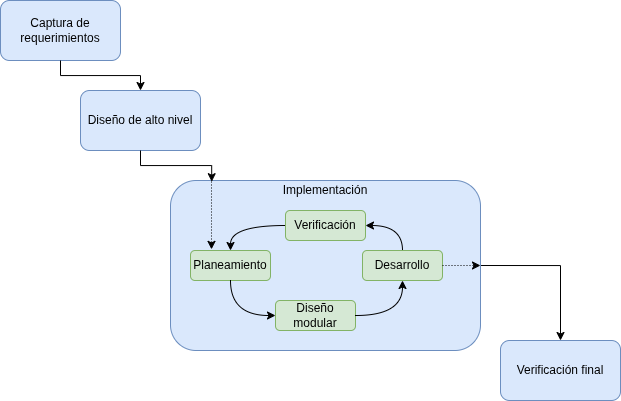
\includegraphics[width=0.8\textwidth]{methodology.png}
    \caption{Proceso metodológico adoptado para el desarrollo del sistema propuesto.}
    \label{fig:metodologia}
\end{figure}

Algunos puntos importantes a considerar en la implementación de este enfoque metodológico son:
\begin{itemize}
    \item Los ciclos de implementación tuvieron una duración de dos semanas.
    \item Cada ciclo incluyó una reunión de planificación con la contraparte de la organización, donde se definió el alcance y las tareas a realizar.
    \item Cada ciclo incluyó una etapa de diseño específica para cada módulo a desarrollar, pero que partió del diseño de alto nivel previamente establecido.
    \item Se mantuvo un tablero virtual al estilo Kanban para el seguimiento del estado de las tareas y el progreso del proyecto.
    \item Al final de cada ciclo se hizo una revisión del trabajo realizado con la contraparte organizacional, las cuales tomaron forma de pruebas de aceptación de usuario o demostraciones del sistema.
    \item En las sesiones de verificación se obtuvo retroalimentación continua, lo que permitió realizar ajustes y mejoras que se reflejaron en los ciclos siguientes.
\end{itemize}

\section{Actividades desarrolladas para cada objetivo específico del proyecto}

En la Tabla \ref{tab:activities} se presenta un desglose de las actividades realizadas para cada uno de los objetivos específicos planteados en la sección \ref{secc:objectives}, junto con sus entregables asociados, técnicas o herramientas utilizadas y estrategias de verificación implementadas. Para mayor facilidad de lectura, se utiliza el identificador de cada objetivo específico:

\objectives

Los entregables asociados a cada objetivo específico se pueden consultar en la Tabla \ref{tab:deliverables}, donde se añadió una breve descripción de cada entregable. Ahora bien, a continuación se enumeran dichos entregables con su respectivo identificador único que será referenciado en la tabla:

\begin{itemize}
    \item \textbf{E1:} \deliverablearch
    \item \textbf{E2:} \deliverabledet
    \item \textbf{E3:} \deliverableos
    \item \textbf{E4:} \deliverablerec
    \item \textbf{E5:} \deliverablerep
    \item \textbf{E6:} \deliverableperf
\end{itemize}

El listado de actividades desarrolladas para alcanzar el cumplimiento de los objetivos específicos del proyecto se presenta a continuación. Cada actividad también está asociada a un identificador único que se utiliza en la tabla para facilitar su referencia:

\begin{itemize}
    \item \textbf{A1-1:} Levantamiento de requisitos del sistema.
    \item \textbf{A1-2:} Selección comparativa de la plataforma de hardware.
    \item \textbf{A1-3:} Diseño de arquitectura física del hardware: mapeo de pines y buses de comunicación.
    \item \textbf{A1-4:} Diseño de arquitectura lógica del sistema.
    \item \textbf{A2-1:} Modelado de la experiencia de usuario y guion de pantallas.
    \item \textbf{A2-2:} Desarrollo del módulo de detección facial en nodo \textit{on-edge}.
    \item \textbf{A2-3:} Integración del módulo de detección facial con la interfaz de usuario.
    \item \textbf{A2-4:} Configuración de Yocto Project y generación de la primera imagen mínima.
    \item \textbf{A2-5:} Personalización de la imagen.
    \item \textbf{A2-6:} Adaptación de base de datos para el registro de accesos.
    \item \textbf{A2-7:} Habilitación de repositorio para almacenamiento de imágenes de los rostros de los usuarios.
    \item \textbf{A2-8:} Desarrollo de servicio \textit{serverless} para el registro de usuarios.
    \item \textbf{A2-9:} Desarrollo de servicio \textit{serverless} para el reconocimiento de usuarios y validación de membresía.
    \item \textbf{A2-10:} Publicación de \textit{endpoints} para utilizar los servicios.
    \item \textbf{A3-1:} Especificación de requisitos de información de reportes de acceso.
    \item \textbf{A3-2:} Implementación de servicios REST para el consumo de reportes de acceso.
    \item \textbf{A3-3:} Desarrollo de la interfaz de usuario para la visualización de reportes.
    \item \textbf{A4-1:} Elaboración del plan de pruebas.
    \item \textbf{A4-2:} Preparación del entorno de pruebas en gimnasio piloto.
    \item \textbf{A4-3:} Ejecución de pruebas de punto a punto del sistema.
    \item \textbf{A4-4:} Análisis estadístico de resultados y comparación con los objetivos de desempeño.
\end{itemize}


\begin{landscape} % Start landscape mode
    \begin{longtable}{l|l|p{2.5cm}|p{7cm}|p{7cm}}
        \caption{Desglose de actividades desarrolladas para cada objetivo específico.} \label{tab:activities} \\
        \hline
        \multicolumn{1}{c|}{\textbf{Obj. Esp.}} & \multicolumn{1}{c|}{\textbf{Entregables}} & \multicolumn{1}{c|}{\textbf{Actividades}} & \multicolumn{1}{c|}{\textbf{Herramientas/Técnicas}} & \multicolumn{1}{c}{\textbf{Estrategias de verificación}} \\ \hline
        \endfirsthead

        \multicolumn{5}{c}{\tablename \thetable{}: Desglose de actividades desarrolladas para cada objetivo específico (continuación).} \\
        \hline

        \multicolumn{1}{c|}{\textbf{Obj. Esp.}} & \multicolumn{1}{c|}{\textbf{Entregables}} & \multicolumn{1}{c|}{\textbf{Actividades}} & \multicolumn{1}{c|}{\textbf{Herramientas/Técnicas}} & \multicolumn{1}{c}{\textbf{Estrategias de verificación}} \\ \hline
        \endhead

        \hline
        \multicolumn{5}{r}{\textit{Continúa en la siguiente página}} \\ \hline
        \endfoot

        \hline
        \endlastfoot

        OE1 & E1 & A1-1, A1-2, A1-3, A1-4 & \vspace{-\baselineskip}
        \setlength{\leftmargini}{1em}
        \begin{itemize}
            \item Entrevistas con partes interesadas para el levantamiento de requisitos.
            \item Revisión de hoja de datos de Raspberry Pi 4B (plataforma disponible en la organización) y de sus posibles alternativas.
            \item Revisión de hoja de datos de cámaras compatibles.
            \item Revisión de hoja de datos de pantalla táctil compatible.
            \item Uso de software Draw.io para diagramas de arquitectura.
        \end{itemize} & \vspace{-\baselineskip}
        \setlength{\leftmargini}{1em}
        \begin{itemize}
            \item Aprobación de los requisitos del sistema por parte de la contraparte de la organización.
            \item Aprobación del documento de arquitectura física y lógica del sistema por parte de la contraparte de la organización.
            \item Verificación que el costo total de la plataforma de hardware no excede los \$300 USD.
        \end{itemize} \\
        \hline

        OE2 & E2, E3, E4 & A2-1, A2-2, A2-3, A2-4, A2-5, A2-6, A2-7, A2-8, A2-9, A2-10 & \vspace{-\baselineskip}
        \setlength{\leftmargini}{1em}
        \begin{itemize}
            \item Generación bosquejo (\textit{mockup}) de interfaz gráfica de usuario usando \textit{Draw.io}.
            \item Uso de \textit{git} para el control de versiones del código fuente. 
            \item Implementación de detección facial con \textit{C++} y \textit{OpenCV}.
            \item Generación de imagen Linux reproducible con \textit{poky} (Yocto).
            \item Orquestación de \textit{builds} con \textit{BitBake} (Yocto).
            \item Activación de capas como \textit{meta-yocto-bsp}, \textit{meta-poky} y \textit{meta-raspberrypi} para definir la plataforma y distribución (Yocto).
            \item Generación de SDK para permitir el desarrollo de aplicaciones sobre la imagen (Yocto).
            \item Creación o modificación de \textit{recipes} y archivos \textit{append} para incluir dependencias y configuraciones específicas (Yocto).
            \item Configuración de caché de estado para acelerar el proceso de compilación mediante el uso de \textit{sstate-cache} (Yocto).
        \end{itemize} & \vspace{-\baselineskip}
        \setlength{\leftmargini}{1em}
        \begin{itemize}
            \item Pruebas de usabilidad con los bosquejos de interfaz gráfica de usuario.
            \item Prueba de despliegue de la imagen Yocto en la Raspberry Pi 4B.
            \item Pruebas unitarias del módulo de detección facial que validan tasa de detección superior al 95\% con un banco de imágenes de referencia.
            \item Pruebas de \textit{endpoints} de servicios REST con \textit{Postman} (tipos de solicitudes, códigos de error, esquema de respuesta).
            \item Pruebas de precisión (mayor al 95\%) y latencia (menor a 500 ms) del servicio  de reconocimiento facial con un banco de imágenes de referencia.
            \item Pruebas de carga y resiliencia: hasta 50 peticiones concurrentes, sin degradación significativa de latencia ni errores 5XX.
            \item Validación de registros de acceso en la base de datos de Fito App.
        \end{itemize}\\
        \hline
        
         & & & \vspace{-\baselineskip}
        \setlength{\leftmargini}{1em}
        \begin{itemize}
            \item Uso de \textit{PostreSQL} para la modificación de la base de datos de Fito App y su adaptación a los requerimientos del sistema.
            \item Configuración de un \textit{bucket} en \textit{Amazon S3} para el almacenamiento de imágenes de rostros.
            \item Configuración de Red de Distribución de Contenidos (\textit{CDN}) para el consumo y distribución de imágenes.
            \item Uso de \textit{AWS Lambda} para el desarrollo de servicios \textit{serverless}.
            \item Uso de \textit{API Gateway} para la creación de \textit{endpoints REST}.
            \item Uso de API de \textit{Amazon Rekognition} para el reconocimiento facial.
            \item Uso de \textit{Python} para el desarrollo de servicios \textit{serverless} y comunicación con APIs.
            
        \end{itemize} & \\
        \hline

        OE3 & E5 & A3-1, A3-2, A3-3 & \vspace{-\baselineskip}
        \setlength{\leftmargini}{1em}
        \begin{itemize} 
            \item Uso de \textit{Node.js}, \textit{Drizzle ORM} y \textit{Neon SDK} para el desarrollo de servicios REST.
            \item Implementación con \textit{React} y \textit{Next.js} para la interfaz de usuario.
        \end{itemize} & \vspace{-\baselineskip}
        \setlength{\leftmargini}{1em} 
        \begin{itemize}
            \item Pruebas de usabilidad de la interfaz de reportes con usuarios administradores para evaluar claridad de las gráficas, tablas y filtros.
            \item Validación de consistencia de datos: comparación de un subconjunto de estadísticas contra los registros de acceso en la base de datos garantizando una desviación menor al 1\%.
            % \item Comprobación de que la paginación y el filtrado por fecha/usuario funcionan correctamente en distintos navegadores y resoluciones.
        \end{itemize}\\
        \hline

        OE4 & E6 & A4-1, A4-2, A4-3, A4-4 & \vspace{-\baselineskip}
         \setlength{\leftmargini}{1em}
         \begin{itemize}
            \item Medición de métricas de latencia en el reconocimiento facial, mediante la librería \texttt{std::chrono} en \textit{C++}.
            \item Registro manual de tasas de aciertos y fallos en el reconocimiento facial.
            \item Implementación de pruebas de aceptación de usuario (\textit{UAT}) con usuarios reales del gimnasio piloto.
            \item Uso de librerías de análisis estadístico y visualización de datos como \textit{Matplotlib} y \textit{NumPy} en \textit{Python} para el análisis de resultados.
         \end{itemize}
        & \vspace{-\baselineskip}
         \setlength{\leftmargini}{1em}
         \begin{itemize}
            \item Revisión del documento de los resultados y análisis por parte de la contraparte de la organización. 
         \end{itemize}\\
        \hline

    \end{longtable}
\end{landscape} % End landscape mode



  % \chapter{Marco metodológico (Cóloque un nombre reprensativo de su proyecto, puede ser un nombre corto)}
\label{ch:solucion}


  % \chapter{Resultados y análisis}


  % \chapter{Conclusiones}

Recordar que las conclusiones no son un resumen de lo que se desarrolló

\section{Recomendaciones}





  %----------------------------------------------------------------------------
  % literature
  \bibliographystyle{IEEEtran}
  \bibliography{references}
  %----------------------------------------------------------------------------

  %----------------------------------------------------------------------------
  % \appendix
  %----------------------------------------------------------------------------

  % \chapter{APENDICE A}
\label{appendix:apendiceA}



\chapter{APENDICE B}
\label{appendix:apendiceB}



\chapter{APENDICE C}
\label{appendix:apendiceC}


  %----------------------------------------------------------------------------
  \backmatter
  %----------------------------------------------------------------------------

  %\printindex                % insert index into document. Don't forget to call
                             % "makeindex filename" first.
\end{document}
